We extend our calculations to the case of N assets. The ultimate goal is to find a combination of weights that minimizes the variance for each level of return we set. We will arrive to show that this can be achieved, and all the portfolio will lie on a parabola in a mean return-variance plane.\\
First we set some notation: let $\mathbf{\Sigma}$ be the covariance matrix of out strategies, it will be a matrix of the form:

$$
\mathbf{\Sigma}_{i,j} = 
\begin{pmatrix}
\sigma_{1}^2 & \rho_{1,2}\sigma_1\sigma_2 & \cdots & \rho_{1,n}\sigma_1\sigma_n \\
\rho_{1,2}\sigma_2\sigma_1 & \sigma_2^2 &   \cdots & \rho_{2,n}\sigma_2\sigma_n \\
\vdots  & \vdots  & \ddots & \vdots  \\
\rho_{n,1}\sigma_n\sigma_1 & \rho_{n,2}\sigma_n\sigma_2 & \cdots & \sigma_n^2 
\end{pmatrix}
$$

While $\mathbf{u}$ will be the vectors of expected returns of each strategy:

$$
\mathbf{u}_{i} = 
\begin{pmatrix}
\mu_1 & \mu_2 & \cdots & \mu_n  
\end{pmatrix}
$$

We will allocate capital expressed in percentage terms expressed by the vector 
$\mathbf{w} = \begin{bmatrix} w_1 & w_2 & \cdots & w_n \end{bmatrix}$ such that $\mathbf{w}^\top \mathbf{1} = 1$.\\
Now it is just about solving a linear optimization problem:

\begin{equation} \label{min_problem}
min \quad \frac{1}{2}\mathbf{w}^\top\mathbf{\Sigma}\mathbf{w} \qquad s.t. \qquad \mathbf{w}^\top \mathbf{1} = 1 \quad \mathbf{w}^\top \mathbf{u} = \bar{\mu}
\end{equation}

Let's write the lagrangean:

\begin{equation} \label{lagrangean}
\mathcal{L} =  \frac{1}{2}\mathbf{w}^\top\mathbf{\Sigma}\mathbf{w} -\xi(\mathbf{w}^\top \mathbf{1} - 1) - \lambda(\mathbf{w}^\top \mathbf{u} - \bar{\mu})
\end{equation}

We can immediately get the F.O.C.s:

\begin{equation} \label{focs}
\begin{split}
\frac{\partial \mathcal{L}}{\partial \mathbf{w}} &= \mathbf{\Sigma}\mathbf{w}  - \xi\mathbf{1} - \lambda\mathbf{u} = 0\\
\frac{\partial \mathcal{L}}{\partial \xi} &= \mathbf{w}^\top \mathbf{1} - 1 = 0\\
\frac{\partial \mathcal{L}}{\partial \lambda} &= \mathbf{w}^\top \mathbf{u} - \bar{\mu} = 0
\end{split}
\end{equation}

From the first F.O.C. we get:

\begin{equation} \label{first_result}
\mathbf{w} = \xi\mathbf{\Sigma}^{-1}\mathbf{1} + \lambda\mathbf{\Sigma}^{-1}\mathbf{u}
\end{equation}

Substituting \eqref{first_result} into the other two F.O.C.s we get the following system of equations:

\begin{equation} \label{focs}
\begin{split}
\xi \mathbf{1}^\top \mathbf{\Sigma}^{-1}\mathbf{1} + \lambda \mathbf{u}^\top \mathbf{\Sigma}^{-1}\mathbf{1} &= 1\\
\xi \mathbf{1}^\top \mathbf{\Sigma}^{-1}\mathbf{u} + \lambda \mathbf{u}^\top \mathbf{\Sigma}^{-1}\mathbf{u} &= \bar{\mu}
\end{split}
\end{equation}

Let's introduce the following notation:
$$
A = \mathbf{u}^\top \mathbf{\Sigma}^{-1}\mathbf{u} \qquad A = \mathbf{u}^\top \mathbf{\Sigma}^{-1}\mathbf{1} \qquad C = \mathbf{1}^\top \mathbf{\Sigma}^{-1}\mathbf{1} \qquad D = AC - B^2
$$

We rewrite the two equations:

\begin{equation} \label{focs_rewritten}
\begin{split}
\xi C + \lambda B &= 1\\
\xi B + \lambda A &= \bar{\mu}
\end{split}
\end{equation}

From which we can easily find that

\begin{equation} 
	\begin{split}
\lambda &= \frac{C\bar{\mu} - B}{D}\\
\xi     &= \frac{A - \bar{\mu}B}{D}
\end{split}
\end{equation}

We can plug this result into \eqref{first_result} to obtain a complete formula for $\mathbf{w}$:

\begin{equation} \label{final_result}
\mathbf{w} = \frac{A - \bar{\mu}B}{D}\mathbf{\Sigma}^{-1}\mathbf{1} + \frac{C\bar{\mu} - B}{D}\mathbf{\Sigma}^{-1}\mathbf{u}
\end{equation}

One can prove that the resulting variance of the portfolio is of the form:

\begin{equation} \label{N_portfolio_variance}
\sigma^2_{\Pi} = \mathbf{w}^\top \mathbf{\Sigma}\mathbf{w} = \frac{C\bar{\mu}^2 - 2B\bar{\mu} + A}{D}
\end{equation}

That is definitely a parabola in the mean return-variance plane. This is called the \textit{Portfolio Frontier} and the upper part of it that has higher return for same variance is referred to as the \textit{Efficient Frontier}.\\
We tried to obtain this empirically, so what we did is to take 20 random strategies (with decent performance) out of our huge dataset and we numerically optimized to find the portfolio frontier for any level of return. We chose 50 strategies that had a performance that lies in the 75th percentile of the ranked performance of strategies. This was done so that we could easily have portfolios with both positive and negative returns, while allowing us to have a reasonably-performing equal weighted portfolio to benchmark against. Of course, our analysis is forward looking in the sense that we computed returns and covariance matrices looking at the whole period. This is done only for pedagogical purposes. Here is the performance of the equally weighted portfolio:

\begin{center}
	\centering
	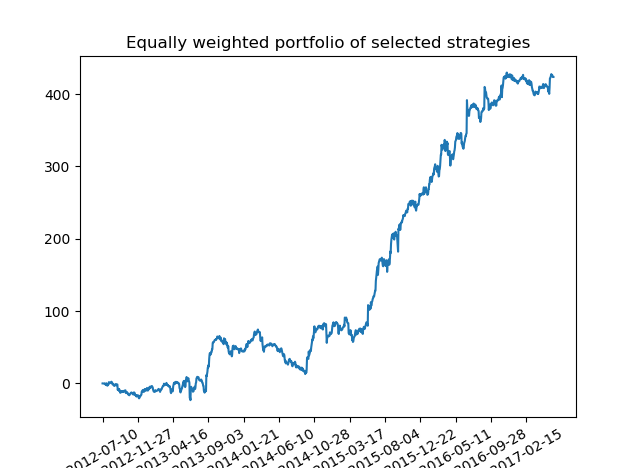
\includegraphics[width=0.6\textwidth]{Portfolio_Theory/Portfolio_Front_Figure_1.png}
	\captionof{figure}{Equally weighted portfolio of 50 strategies in the 75th percentile in terms of performance}
	\label{Equal_Weight_frontier}
\end{center}


It's sharpe is about 1.37, nothing special but at least it acts as a decent benchmark. Now let's try to build an efficient frontier from the calculations made before. We obtain the following efficient frontier in the $\sigma^2-\mu$ plan:

\begin{center}
	\centering
	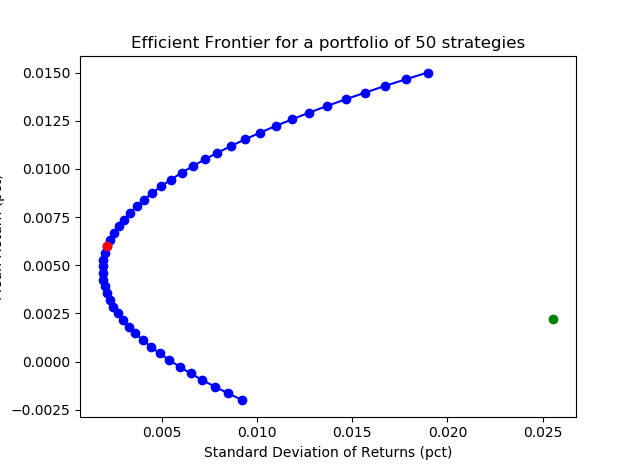
\includegraphics[width=0.6\textwidth]{Portfolio_Theory/Portfolio_Front_Figure_2.png}
	\captionof{figure}{Resulting portfolio frontier}
	\label{Frontier_frontier}
\end{center}

First of all we can spot the traditional parabolic shape of the portfolio frontier. The upper part of the portfolio frontier is referred to as the \textit{Efficient Portfolio Frontier}. We also highlighted two portfolios: the maximum Sharpe-ratio portfolio (red marker) and the equally weighted portfolio (green marker). We can clearly see how the equally weighted portfolio is non-optimal, with the same level of return we can substantially reduce our risk by finding a relative efficient allocation. The red spot is an interesting point, this portfolio is the one that achieves the maximum Sharpe-ratio, or in other words it provides the best tradeoff between risk and return. This portfolio can be obtained by analytical derivations, but in this case we just looked into the set of portfolios that we generated. In our project we will try to make our portfolio resemble this optimal one out-of-sample.\\
One important remark should be made before we move on: we will not be able to achieve the same level of optimality as we will not have the luxury of forecasting returns and variances.